
随机库提供了选择的随机数生成器,每个生成器具有不同的策略和属性。本节中,我们检查一个函数,通过创建输出的直方图来比较不同的选项。

\subsubsection{How to do it…}

这个示例中,比较了C++随机库提供的不同随机数生成器:

\begin{itemize}
\item 
从一些常量开始,为随机数生成器提供统一参数:

\begin{lstlisting}[style=styleCXX]
constexpr size_t n_samples{ 1000 };
constexpr size_t n_partitions{ 10 };
constexpr size_t n_max{ 50 };
\end{lstlisting}

n\_samples是要检查的样本数量,n\_partitions是用来显示样本的分区数量,n\_max是直方图中条形图的最大值(由于四舍五入的关系,这个值会有所变化)。

这些数字合理地显示了引擎之间的差异。增加样本与分区的比例往往会使曲线变得平滑,并模糊引擎之间的差异。

\item 
这是一个收集随机数样本并显示直方图的函数:

\begin{lstlisting}[style=styleCXX]
template <typename RNG>
void histogram(const string_view& rng_name) {
	auto p_ratio = (double)RNG::max() / n_partitions;
	RNG rng{}; // construct the engine object
	
	// collect the samples
	vector<size_t> v(n_partitions);
	for(size_t i{}; i < n_samples; ++i) {
		++v[rng() / p_ratio];
	}

	// display the histogram
	auto max_el = std::max_element(v.begin(),
		v.end());
	auto v_ratio = *max_el / n_max;
	if(v_ratio < 1) v_ratio = 1;
	cout << format("engine: {}\n", rng_name);
	for(size_t i{}; i < n_partitions; ++i) {
		cout << format("{:02}:{:*<{}}\n",
			i + 1, ' ', v[i] / v_ratio);
	}
	cout << '\n';
}
\end{lstlisting}


简而言之,这个函数将收集的样本的直方图存储在一个vector中。然后,在控制台上以星号的形式显示直方图。

\item 
在main()使用histogram(),如下所示:

\begin{lstlisting}[style=styleCXX]
int main() {
	histogram<std::random_device>("random_device");
	histogram<std::default_random_engine>
		("default_random_engine");
	histogram<std::minstd_rand0>("minstd_rand0");
	histogram<std::minstd_rand>("minstd_rand");
	histogram<std::mt19937>("mt19937");
	histogram<std::mt19937_64>("mt19937_64");
	histogram<std::ranlux24_base>("ranlux24_base");
	histogram<std::ranlux48_base>("ranlux48_base");
	histogram<std::ranlux24>("ranlux24");
	histogram<std::ranlux48>("ranlux48");
	histogram<std::knuth_b>("knuth_b");
}
\end{lstlisting}

输出为:

\begin{center}
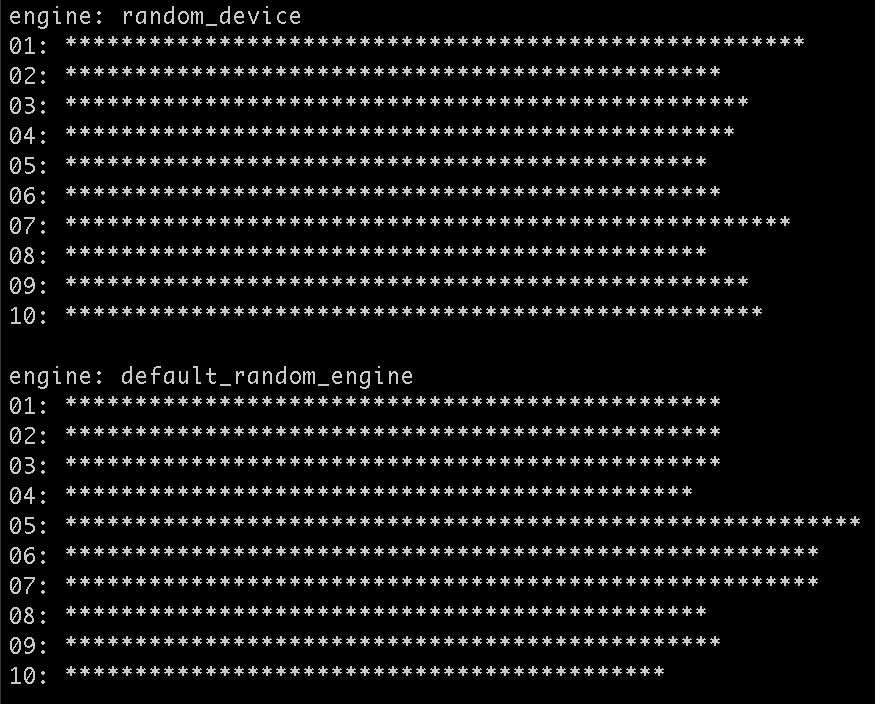
\includegraphics[width=0.6\textwidth]{content/chapter8/images/1.png}\\
图8.1 前两个随机数引擎输出的截图
\end{center}

截图显示了前两个随机数引擎的直方图。

若将n\_samples的值提高到100,000,会发现引擎之间的差异变得更难辨别:

\begin{center}
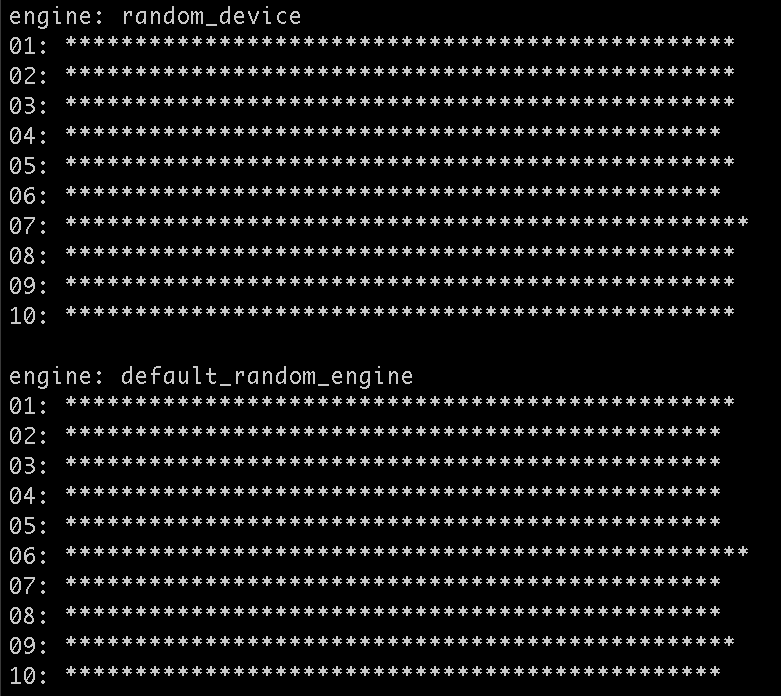
\includegraphics[width=0.6\textwidth]{content/chapter8/images/2.png}\\
图8.2  100,000个样本的输出截图
\end{center}

\end{itemize}

\subsubsection{How it works…}

每个随机数引擎都有一个函子接口,返回序列中的下一个随机数:

\begin{lstlisting}[style=styleCXX]
result_type operator()();
\end{lstlisting}

函子会返回一个随机值,平均分布在min()和max()值之间。所有的随机数引擎都有这个接口。

histogram()函数可以通过在模板中使用随机数引擎类,来利用这种一致性:

\begin{lstlisting}[style=styleCXX]
template <typename RNG>
\end{lstlisting}

(RNG是随机数生成器(Random Number Generator)的缩写。标准库文档将这些类称为引擎,就我们的目的而言,这与RNG同义。)

我们用RNG类实例化一个对象,并在vector中创建一个直方图:

\begin{lstlisting}[style=styleCXX]
RNG rng{};
vector<size_t> v(n_partitions);
for(size_t i{}; i < n_samples; ++i) {
	++v[rng() / p_ratio];
}
\end{lstlisting}

使用这种方式,可以很容易地比较各种随机数引擎的结果。


\subsubsection{There's more…}

库中的每个随机数引擎都有不同的方法和特征。当多次运行直方图时,会注意到大多数引擎在每次运行时都具有相同的分布,因为它们是确定的——每次生成相同的数字序列。std::random\_device在大多数系统上是不确定的。若需要更多的变化,可以使用它为其他引擎生成随机种子。使用当前日期和时间为RNG种子的情况也很常见。

std::default\_random\_engine对于多数情况来说都是一个合适的选择。


















